\begin{figure*}

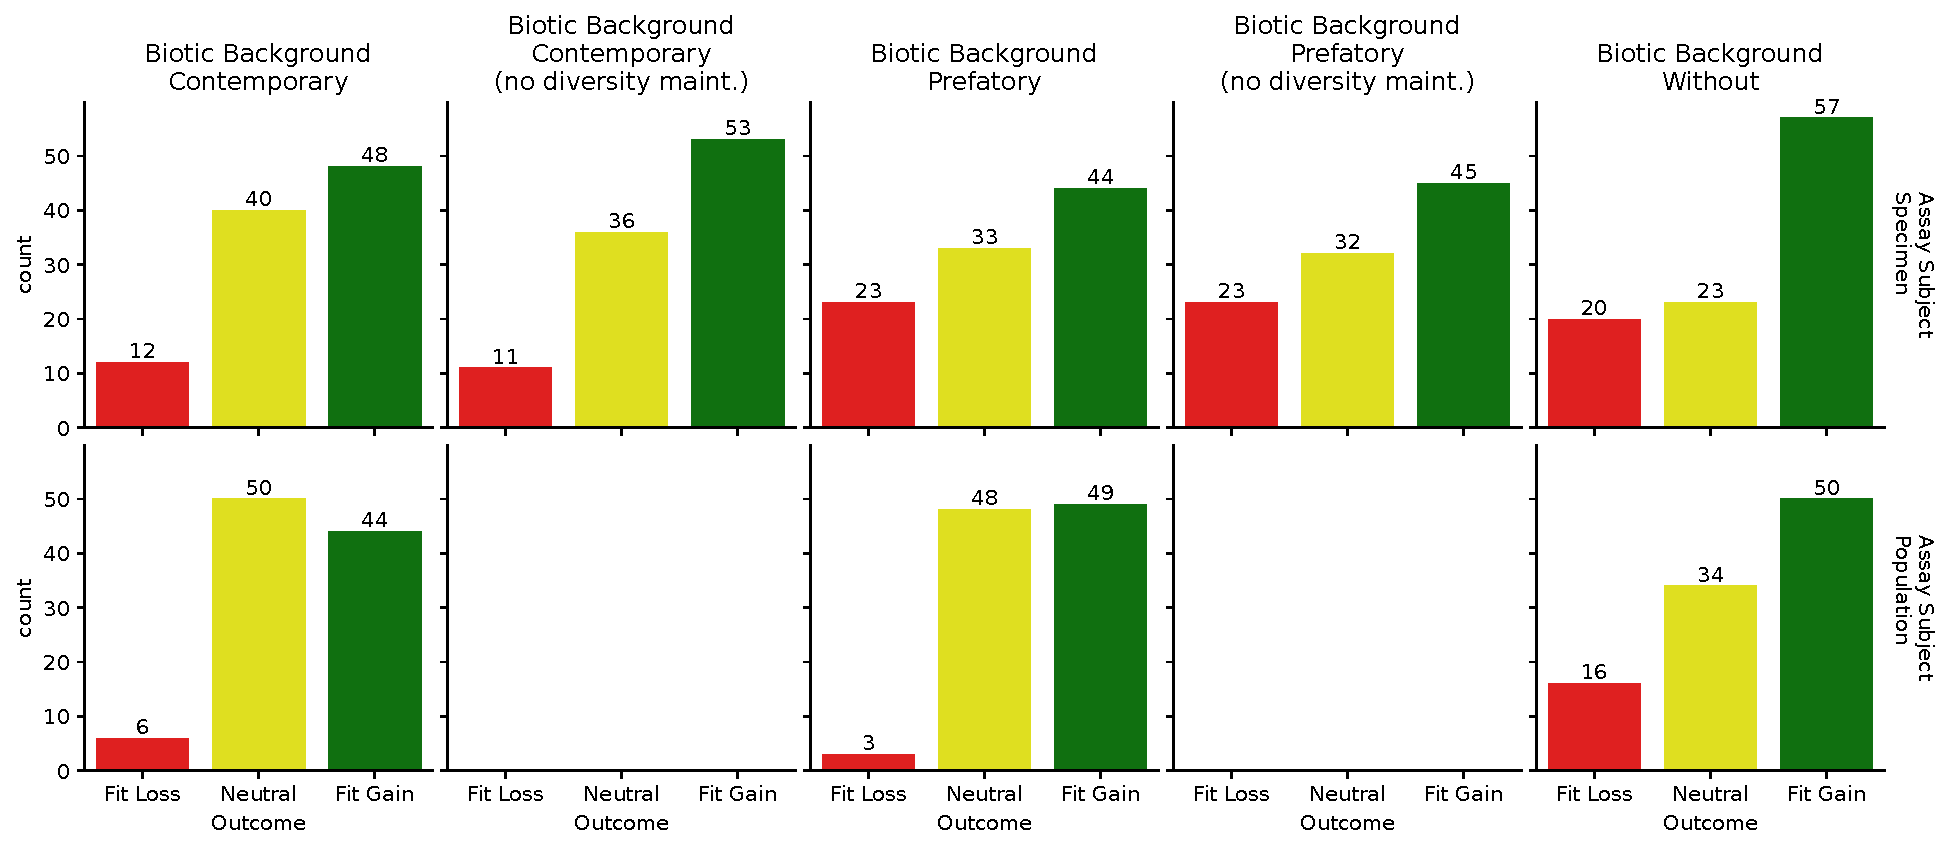
\includegraphics[width=\linewidth]{{submodule/dishtiny/binder/bucket=prq49/a=adaptation_assays+endeavor=16/teeplots/col=biotic-background+kind=count+row=assay-subject+viz=barlabel-catplot+x=outcome+ext=}}

\caption{
\textbf{Distribution of adaptation assay outcomes.}
\footnotesize
For each adaptation assay, three outcomes were possible: significant fitness gain, significant fitness loss, or no significant fitness change (``neutral'').
Significance cutoff $p < 0.005$ was used.
A fitness loss --- color-coded red --- corresponds to winning 2 or fewer competitions out of 20 against the preceding stint's focal strain population.
A fitness gain --- color-coded green --- corresponds to winning 18 or more competitions out of 20 against the preceding stint's focal strain population.
Neutral fitness outcomes are color-coded yellow.
Outcome counts are accumulated over experiments from stint 1 through stint 100.
Upper row shows results for sampled focal strain genome, lower row shows results for entire focal strain population.
See Figure \ref{fig:adaptation_assay_cartoon} for explanation of competition biotic backgrounds.
See Figure \ref{fig:outcome_count_joint_distns} for joint distributions of fitness outcomes across biotic backgrounds.
}
\label{fig:outcome_count_distns}
\end{figure*}
